
%\documentclass[10pt,twoside,twocolumn]{article}
\documentclass[10pt,twoside]{article}
\usepackage[bf,small]{caption}
\usepackage[letterpaper,hmargin=1in,vmargin=1in]{geometry}
\usepackage{paralist} % comapctitem, compactdesc, compactenum
\usepackage{titlesec}
\usepackage{titletoc}
\usepackage{times}
\usepackage{hyperref}
\usepackage{algorithmic}
%\usepackage{glossaries}
%\usepackage[xindy]{glossaries}
%\usepackage[toc]{glossaries}
\usepackage{graphicx}
\graphicspath{{./graphics/}}
\usepackage{xspace}
\usepackage{verbatim}
\hyphenation{Sub-Bytes Shift-Rows Mix-Col-umns Add-Round-Key}

\setlength{\parskip}{10pt}
\setlength{\parindent}{0pt}

\newcommand{\sh}{\emph{sector\_hash}\xspace}
\newcommand{\hdb}{\texttt{hashdb}\xspace}
\newcommand{\bulk}{\emph{bulk\_extractor}\xspace}
\newcommand{\mdd}{\emph{md5deep}\xspace}

\begin{document}

%\titlespacing{\section}{0pt}{0pt}{0pt}
%\titlespacing{\subsection}{0pt}{0pt}{0pt}
%\titlespacing{\subsubsection}{0pt}{0pt}{0pt}
%\date{}
\title{Hash (\sh) Tool Summary}
\author{Bruce Allen \footnote{\href{mailto:bdallen@nps.edu}{bdallen@nps.edu}}}
\maketitle

\begin{abstract}
The Hash (\sh) tool
provides facilities for creating a hash database (\hdb)
of MD5 hashes on files along chunk boundaries
as well as querying hash datasets,
merging hash datasets,
and allowing hash lookups.
Multiple map types are supported, allowing for specific optimizations.
The \hdb may be imported and exported in DFXML format~\cite{dfxml}.
\end{abstract}

%%\newpage
%\cleardoublepage
%\setcounter{tocdepth}{2}
%\tableofcontents
%%\newpage
%\cleardoublepage

\section{Introduction}
Hash databases are useful for quickly determining if content 
is whitelisted or blacklisted.
A hash database contains hashes of chunks of data.
A \emph{chunk} is a contiguous sequence of bites of some fixed size.  Since data to be
hashed can come from any source, we don't call the sequences of bytes
\emph{sectors} or \emph{blocks}. 
A hash database built from chunks 
allows detection of one-time presense of content even if only one chunk of that
content is currently present; whereas if only a single byte was changed, a file
hash database would not be useful for detecting the presense of the content.
In this document, we present the requirements for building a toolset for
constructing, managing, and querying hash databases built from chunks of data.
We call the overall database the ``\hdb''.

The envisioned workflow for creating and using a \hdb is as follows:
\begin{compactenum}
\item Generate a \hdb of MD5 hashes.
      An MD5 hash is generated for each chunk sourced,
      and is stored within the \hdb for future lookup.
      Chunks are typically 4K in size.
\item Search a piece of media or data stream for hash values that match those in a \hdb.
      Specifically, generate MD5 hash values for chunks take from
      the input media or stream
      and query to see if the generated hash values match any of the hash values in the \hdb.
\end{compactenum}

\section{The Hash Database (\hdb)}
A hash database (\hdb) contains a database of hash values along with information
identifying from where the hash values were sourced.
The \hdb structure is shown in Figure~\ref{fig-hashdb}.
Specifically, a \hdb consists of the following components:
\begin{compactitem}
\item Metadata about the hash database.
\item The hash store mapping chunk hash values to source lookup records.
\item A hash duplicates store mapping duplicate chunk hash values to multiple source lookup records.
\item The source lookup store mapping source lookup index values to source locations.
\item Up to two Bloom filters, used internally for optimizing performance
      when searching for hash values that might be present in the hash store.
\end{compactitem}
A \hdb is stored as a directory containing the following files:
\begin{compactitem}
\item \texttt{hashdb\_metadata.xml}
\item \texttt{hash}
\item \texttt{hash\_duplicates}
\item \texttt{source\_lookup}
\item \texttt{bloom1}
\item \texttt{bloom2}
\end{compactitem}
Filenames vary depending on tuning preferences (see Section\ref{tuning}). 
\begin{compactitem}
  \item Sharding of the \texttt{hash} file is supported for hash value lookups.
        Shard files provide prefix routing on \begin{math}2^{n}\end{math} choices based
        on the lead bits of the MD5 hash.
        Each shard will in a separate file with filename extensions consisting of the
        decimal representation of the prefix, front padded with zeros to a common
        length.  For example with a four-bit prefix, the extensions are ``.01'',
        ``.02'', ... ``.15''. 
  \item In the future we may decide to also shard the 
        the \texttt{bloom1} and \texttt{bloom2} files.  For example, file \texttt{bloom1.01}
        would be built from only the hashes stored in file \texttt{hash.01}.
  \item Files \texttt{bloom1} and \texttt{bloom2} are only present when Bloom
        filters are being used.
\end{compactitem}

\begin{figure}[h]
  \center
  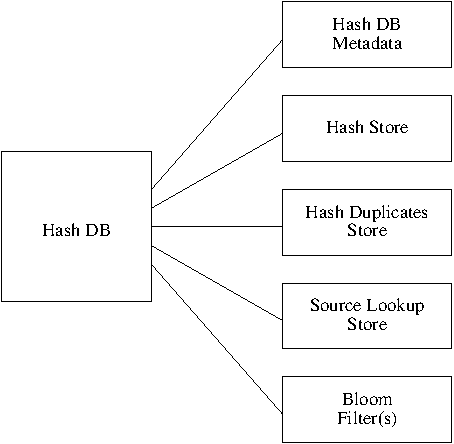
\includegraphics{images/hash_db}
  \caption{Components of the \hdb.\label{fig-hashdb}}
\end{figure}

\subsection{\hdb Metadata\label{hashdb-metadata}}
The \hdb metadata file (\texttt{hashdb\_metadata.xml}) includes the following information:
\begin{compactitem}
\item The map type that is being used for the hash store and the source lookup store,
      see Section~\ref{tuning-map-type}
\item The number of elements in the hash store.
\item The maximum number of elements in the hash store.
\item The fullness of the hash store (tree-based maps
have a measure of fullness for the nodes within them).
\item The source lookup record type used in the hash store,
see Section~\ref{tuning-source-lookup-record-type}
\item The number of elements in the source lookup store.
\item The maximum number of elements in the source lookup store.
\item The number of Bloom filter hash functions \emph{k}
and the size of the Bloom filter hash \emph{m} for each Bloom filter,
see Section~\ref{tuning-bloom-filter}
\item Map size, map fragmentation, or other parameters
that may only apply to specific to map types in use.
\end{compactitem}
The \hdb metadata is in DFXML format \cite{dfxml}.

\subsection{Hash Store}
The hash store contains all the MD5 hash values in the hash database
along with source lookup records required for mapping hash values
to the repository name and filename from which the hash values were sourced.
A diagram of the hash store is shown in Figure~\ref{fig-hash-store}.

\begin{figure}[h]
  \center
  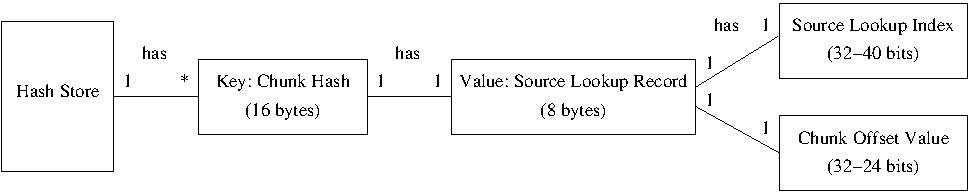
\includegraphics{images/hash_store}
  \caption{Components of the hash store.\label{fig-hash-store}}
\end{figure}

Elements in the hash store contain the following:
\begin{compactitem}
\item \emph{key: chunk hash}: The 16-byte (128-bit) MD5 hash value.
\item \emph{value: source lookup record}: The location from which the chunk was sourced
for calculating the hash.
The \emph{source lookup record} is encoded in two parts:
\begin{compactenum}
\item \emph{source lookup index}: An integer which maps to where the chunk was sourced.
This integer is used as the \emph{key} in the source lookup store
for identifying the repository name and filename
from which the hash was sourced, see Section~\ref{source-lookup-store}.
\item \emph{chunk offset value}: An integer indicating the chunk offset into the block in the file
from which the MD5 hash was sourced.
\end{compactenum}
\end{compactitem}
If the chunk hash is sourced from more than one file,
the source lookup record is set to \texttt{MAX\_VALUE}
and the chunk hash element is stored in the hash duplicates store,
see Section~\ref{hash-duplicates-store}.

\subsection{Hash Duplicates Store\label{hash-duplicates-store}}
A hash duplicates store is required for managing duplicate chunk hash values.
Duplicate chunk hash values can be present as a result of the following conditions:
\begin{compactitem}
\item A file is sourced from more than one place.
\item A file being sourced has already been sourced from the same file
but from a different path, filename, or repository.
\item Although the files are different, a chunk in the file resolves to the same hash as a chunk sourced from another file.
This is common when a file such as a .pdf file has embedded chunks
that are common to other .pdf files.
\end{compactitem}
When there are chunk hash duplicates,
hash elements are stored in the hash duplicates store rather than in the hash store.
Chunk hash duplicates have two or more file lookup records associated with them.
A diagram of the hash duplicates store is shown in Figure~\ref{fig-hash-duplicates-store}.

\begin{figure}[h]
  \center
  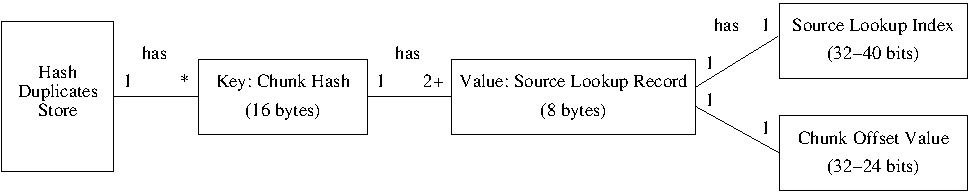
\includegraphics{images/hash_duplicates_store}
  \caption{Components of the hash duplicates store.\label{fig-hash-duplicates-store}}
\end{figure}

\subsection{Source Lookup Store\label{source-lookup-store}}
The source lookup store provides the repository name and filename information
for source lookup indexes that are defined.
A diagram of the source lookup store is shown in Figure~\ref{fig-source-lookup-store}.

The source lookup store contains all the source lookup elements.
Each source lookup element provides the following:
\begin{compactitem}
\item \emph{source lookup index}: A 64-bit field
that maps to a particular source location record.
Note that in the hash store and in the hash duplicates store,
this source lookup index is a 32-40 bit field.
\item \emph{source location record}: A record describing the lookup source.
The record is of variable length and contains the following:
\begin{compactitem}
\item A repository name identifying where sourced filenames were obtained.
By default, this name is the filename of the DFXML file generated
when sourcing chunk hash values using the \mdd message digest tool.
\item The filename as an absolute path on the drive where the sourced file is stored.
\end{compactitem}
\end{compactitem}

\begin{figure}[h]
  \center
  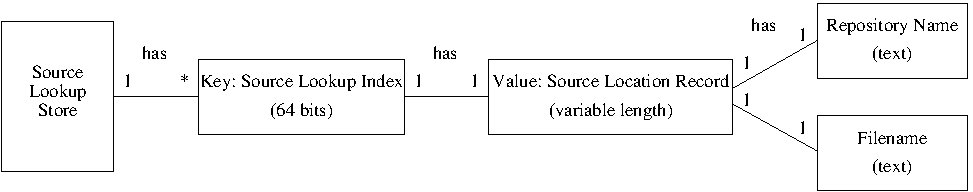
\includegraphics{images/source_lookup_store}
  \caption{Components of the source lookup store.\label{fig-source-lookup-store}}
\end{figure}

\subsection{Bloom Filter Data Structure}
The Bloom filter is a probabilistic data structure used
for increasing the average speed of looking up hash values
when many of the hash values to be looked up are not present in the hash store.
Use of a Bloom filter is optional.
Bloom filters are effective because they can quickly tell if a hash value is not in the hash store.
Consulting a Bloom filter can avoid the higher cost of a map lookup.
A second, cascaded Bloom filter may be used to improve performance further.
See Section~\ref{tuning-bloom-filter} for information on tuning Bloom filters.

\section{Tuning\label{tuning}}
Hash databases are large and have performance limitations.
This section describes the parameters that tune the various components of the \hdb.
The syntax for selecting tuning options using the \sh utility is shown in Section~\ref{usage}.

\subsection{Maps\label{tuning-map-type}}
Various types of map algorithms are available
for managing data stores within the \hdb.

Some map algorithms require specific tuning parameters.
For example some map types require their size to be preallocated.
When building a map, their size should be larger than the number of entries they will hold,
for example 25\% larger.
When reading a map, some map types can be packed down to the size of the number of entries in them.

Not all map types can support all types of data stores within the \hdb.
Specifically:
\begin{compactitem}
\item The hash store supports \emph{Map} types because it has unique keys.
The hash store has fixed-sized fields.
\item The hash duplicates store supports \emph{Multimap} types because it has multiple keys.
The hash duplicates store has fixed-sized fields.
\item The source lookup store supports \emph{Map} types because it has unique keys.
It has variable-sized \emph{value} fields.
\end{compactitem}

\subsubsection{\emph{Map} Types}
The hash store accepts \emph{Map} types.
Supported \emph{Map} types follow:
\begin{compactitem}
\item \emph{red-black tree}:
Provides reasonable performance during construction and usage.
\begin{compactitem}
\item Provides \begin{math}{O(log(n))}\end{math} performance during construction and usage.
\item Can incur processor cache misses along nodes during tree traversal,
requiring additional disk drive accesses.
\item No memory overhead in data density.
\item Memory overhead in managing nodes.
\item Implemented as \texttt{MAP},
see file \texttt{boost/interprocess/containers/map.hpp}.
\end{compactitem}
\item \emph{sorted vector}:
Provides bad performance.
\begin{compactitem}
\item Provides \begin{math}{O(n)}\end{math} performance, worst case, during construction and usage.
\item This algorithm provides forward and reverse iterators, which we do not need.
\item Incurs processor cache misses along nodes during sequential traversal,
requiring additional disk drive accesses.
\item No memory overhead in data density.
\item Memory overhead in managing doubly-linked lists.
\item Implemented as \texttt{FLAT\_MAP},
see file \texttt{boost/interprocess/containers/flat\_map.hpp}.
\end{compactitem}
\item \emph{hash map}:
Provides good performance until the hash store starts to become full.
\begin{compactitem}
\item Provides \begin{math}{O(1)}\end{math} performance unless there are hash collisions.
Because of the random distribution of MD5 hash values, average hash map hash collisions
are well below \begin{math}{O(log(n))}\end{math} when the hash map is less than 70\% full.
\item Incurs processor cache misses for each hash collision.
This can be mitigated by using Linear Probing to find and allocate an adjacent bucket
when there is a map collision.
\item Memory overhead in allocating extra hash map buckets.
\item There is a significant cost in increasing the hash map size
if excessive hash collisions indicate that the hash map size must be increased.
Note: if Linear Probing is used, it is required that there be less entries than buckets.
\item Implemented as \texttt{UNORDERED\_MAP},
see file \texttt{boost/unordered/unordered\_map.hpp}.
\end{compactitem}
\item \emph{btree}:
Similar to \emph{red-black tree}.  It is faster and it wastes memory
because it stores multiple entries per node.
\begin{compactitem}
\item Provides \begin{math}{O(log[q](n))}\end{math} performance during construction and usage,
where \begin{math}q\end{math} is the number of entries per node (this fact needs to be validated).
\item Can incur processor cache misses along nodes during tree traversal,
requiring additional disk drive accesses.
\item No memory overhead in data density.
\item Additional memory overhead in managing pointers for unused entries in nodes.
\item Implemented as \texttt{BTREE\_MAP},
see file \texttt{boost/btree/map.hpp}.
\end{compactitem}
\end{compactitem}

\subsubsection{\emph{Multimap} types\label{tuning-multimap-type}}
The hash duplicates store requires a Multimap.
Multimap implementations similar to map implementations are available:
\begin{compactitem}
\item \emph{red-black tree}, implemented as \texttt{MULTIMAP}, see file \texttt{boost/?.hpp}.
\item \emph{sorted vector}, implemented as \texttt{FLAT\_MULTIMAP}, see file \texttt{boost/?.hpp}.
\item \emph{hash map}, implemented as \texttt{UNORDERED\_MULTIMAP}, see file \texttt{boost/?.hpp}.
\item \emph{btree}, implemented as \texttt{BTREE\_MULTIMAP}, see file \texttt{boost/?.hpp}.
\end{compactitem}

\subsubsection{Map types with Variable \emph{value} Field Size}
The source lookup store
contains elements whose \emph{value} field are of a variable length.
Although any of the four Map types can be used to implement the source lookup store,
we only support one type because
maximum performance is not required
and this map type is the only one that can be written out to a large file (map to?)
as-is without modification:
\begin{compactitem}
\item \emph{btree}, implemented as \texttt{VAR\_VAL\_BTREE\_MAP}, see file \texttt{boost/?.hpp}.
\end{compactitem}

\subsection{Source Lookup Record Types\label{tuning-source-lookup-record-type}}
Another tuning parameter is the structure of the source lookup record
which contains the source lookup index and the chunk offset value.
The source lookup record is used in the hash store, Figure~\ref{fig-hash-store},
and in the hash duplicates store, Figure~\ref{fig-hash-duplicates-store}.
The data structure for the source lookup record is shown in Section~\ref{source-lookup-record}.
Its size is 8 bytes.
For computational performance,
it is effective for the source lookup index and chunk offset value fields
to be 32 bits each.
Unfortunately, the source lookup index can require more than \begin{math}2^{32}\end{math} bits
to fully identify it.
To support this, we provide source lookup record types that provide
between 32 and 40 bits for the source lookup index
and between 32 and 24 bits for the chunk offset value.
Whatever the selection, these fields must be large enough to hold all possible values.

The following tuning option is available:
\begin{compactitem}
\item sliding hash source lookup record value, from 32 to 40.
For example a sliding value of 35 allots bits as follows:
\begin{compactitem}
\item \begin{math}2^{35}\end{math} bits for the source lookup index.
\item \begin{math}2^{29}\end{math} bits for the chunk offset value.
\end{compactitem}
\end{compactitem}

\subsection{Sharded Files}
In the future, the \texttt{hash} file may be split into shards.
Each shard will reside in a file, and the filename will end in extension .01, .02, .03, etc,
indicating the shard number.
Shard files provide prefix routing on \begin{math}2^{n}\end{math} choices.
Individual shard files allow parallel lookups in a distributed processing environment,
where a given processor searches only for hashes within its respective range.
It is only effective to use shard files when they are small enough
to fit within the address space of the processors that are accessing them.

As an optimization, the \texttt{bloom1} and \texttt{bloom2} files may be split,
one for each shard file.
If file lookup optimization is required when sharding,
the \texttt{hash\_duplicates} file may also be split,
one file for each shard file.

\subsection{Bloom Filter\label{tuning-bloom-filter}}
The Bloom filter store is a collection of bit fields.
Sector hash values map to bit positions in the Bloom filter store.
When specific bit positions are set,
this indicates that a sector hash value may have been mapped
to the Bloom filter store.
When specific bit positions are not set,
this indicates that a sector hash value has not been mapped
to the Bloom filter store.
We use this property to determine when sector hash values
have not been added to the hash store.
Specifically, Bloom filters check for the absence of sector hash values
rather than performing hash store lookups directly because, on the average, this is faster.
The Bloom filter works as follows:
\begin{compactenum}
\item Apply \emph{k} Bloom filter hash functions of size \emph{m} bits on the chunk hash value
to be hashed into the Bloom filter.
Since the chunk hash value has high entropy, we simply map bits of the chunk hash value
onto bits of the \begin{math}k*m\end{math} Bloom filter hash function bits.
Since chunk hashes are 128 bits wide, \emph{k} and \emph{m} must be set such that
\begin{math}k*m\le128\end{math}.
\item For each \emph{k}:
\begin{compactenum}
\item Demultiplex \emph{k} to a bit position.
\item Check or set the bit at the demultiplexed bit position,
depending on whether reading or writing.
\end{compactenum}
\end{compactenum}

Bloom filters use the following parameters:
\begin{compactitem}
\item \emph{k}: The number of Bloom filter hash functions to use.
Increased \emph{k} reduces false positives but saturates the filter more quickly.
\item \emph{M}: The size of the Bloom filter hash, in bits.
\item \emph{m}: The size of the Bloom filter, in bits, where \begin{math}m=2^{M}\end{math}.
\item \emph{n}: The number of chunk hash values recorded in the hash store.
\end{compactitem}
When too many sector hash values have been added to the Bloom filter,
it becomes saturated and stops improving performance
because the false positive rate becomes too high.
The false positive rate, \begin{math}P_{fp}\end{math}, may be calculated
using the equation \begin{math}P_{fp}=(1-e^{-kn/m})^k\end{math}.

When the size of the Bloom filter is increased, it has more capacity,
but takes up more disk space.
Disk space consumed, in bytes \emph{B}, is calculated
using the equation \begin{math}B=2^{M-3}\end{math}.

Table~\ref{bloom-parameters} shows example tuning parameters
that may be used to achieve various false positive rates given \emph{n} hashes.

\begin{table}[h]
\center
\begin{tabular}{|c|c|c|c|c|}
\hline
\emph{k} & \emph{M} & \emph{n} & \begin{math}P_{fp}\end{math} & disk space consumed \\
\hline
4 & 32 & \begin{math}1*10^{9}\end{math} & 13.48\% & 512MiB \\
3 & 32 & \begin{math}1*10^{9}\end{math} & 70.60 or 12.70\% & 512MiB \\
3 & 33 & \begin{math}1*10^{9}\end{math} & 0.75 or 2.56\% & 1GiB \\
3 & 34 & \begin{math}1*10^{9}\end{math} & 0.07 or 0.41\% & 2GiB \\
4 & 30 & \begin{math}1*10^{9}\end{math} & 90.70\% & 128MiB \\
\hline
\end{tabular}
\caption{Available Bloom filter configurations and their associated costs.\label{bloom-parameters}}
\end{table}

The following Bloom filter settings are available:
\begin{compactitem}
\item \emph{none}: Do not use a Bloom filter for optimizing chunk hash lookups.
\item \emph{kNN}: Provide the number of hash functions to use.
\item \emph{MNN}: Provide the size of the hash function, in bits.
\end{compactitem}

\subsection{Second Bloom Filter}
Additional performance gain can be achieved by using a second Bloom filter.
The second Bloom filter provides a second check
in an effort to prevent false lookup attempts in the hash store, as follows:
\begin{algorithmic}
\IF{small Bloom filter (\texttt{bloom1}) indicates the hash may be in the hash store}
  \IF{large Bloom filter (\texttt{bloom2}) indicates the hash may be in the hash store}
    \STATE look for the hash in the hash store
  \ENDIF
\ENDIF
\end{algorithmic}

\section{\sh Utility}
The \sh utility performs the various functions relating to managing and accessing MD5 datasets.
The following subcommands are supported:
\begin{compactitem}
\item \texttt{import}:
Create a new \hdb by importing hash data from a DFXML file.
Note that the DFXML file is typically generated using the \mdd utility,
for example \texttt{md5deep -p 4096 -d -r mydir}.
\item \texttt{export}:
Export a \hdb to a DFXML file.
\item \texttt{merge}:
Merge two {\hdb}s formatted with any tuning parameters
into one of the {\hdb}s.
Technical note: source lookup indexes are retained for the modified \hdb
and regenerated for the input \hdb.
\item \texttt{remove}:
Remove entries in the second \hdb from the first \hdb.
\item \texttt{convert}:
Convert a \hdb into a new \hdb formatted with the specified tuning parameters.
\item \texttt{stat}:
Display metadata corresponding to the specified \hdb.
\hdb metadata is described in Section~\ref{hashdb-metadata}.
\item \texttt{lookup}:
Check to see if any chunks of data from stdin
have hash values that match hash values in the \hdb.
For hash values that match, send the chunk offset and source information to stdout.

Example Usage:

\texttt{sector\_hash lookup -i mystorefile < myhashlistfile > mylookupoutput}.

\item \texttt{testwrite}:
This test subcommand creates a test \hdb
filled with the requested quantity of randomly generated entries.
\item \texttt{testread}:
Tests timing performance of reading a \hdb.
\end{compactitem}

\subsection{Usage\label{usage}}
The \sh utility supports the following usage:
\begin{small}
\begin{verbatim}
  Usage: sector_hash -h | -V | [<subcommand>]
      -h      - print this message
      -V      - print version number
  Subcommands:
      import -i <DFXML file> [-n <repository name>] [-a] -o <hashdb>
             [-t <tuning parameter>]+
      export -i <hashdb> -o <DFXML file>
      merge -m <hashdb> -i <hashdb2>
      remove -m <hashdb> -i <hashdb2>
      convert -i <hashdb> -o <hashdb> [-t <tuning parameter>]+
      stat -i <hashdb>
      lookup -i <hashdb>    - uses stdin and stdout streams
      server -i <hashdb>    - starts sector_hash as a lookup server service

  Options:
      -i <input path>       - DB Input path
      -m <input path>       - Path to the DB that is to be modified
      -n <repository name>  - Name of repository from which chunk hashes are sourced
      -o <output path>      - Output path
      -a                    - Add input to an existing output
      -t <tuning parameter> - May be repeated, where <tuning parameter> may be one of:
              hash store type:            hred-black-tree | hsorted-vector
                                          | hunordered-map | hbtree-map
              hash store size:            h<NN>
              hash duplicates store type: dred-black-tree | dsorted-vector
                                          | dunordered-map | dbtree-map
              hash duplicates store size: d<NN>
              source lookup record type:  r<NN>
                                          - where NN is between 32 and 40
              source lookup store type:   sboost-bimap
              source lookup store size:   s<NN>
              Bloom filter 1 ensabled:    b1e
              Bloom filter 1 disabled:    b1x
              Bloom filter 1 functions:   b1k<NN>
              Bloom filter 1 hash size:   b1M<NN>
              Bloom filter 2 ensabled:    b2e
              Bloom filter 2 disabled:    b2x
              Bloom filter 2 functions:   b2k<NN>
              Bloom filter 2 hash size:   b2M<NN>

  Debugging:
      testwrite -o <hashdb> -x <xml outfile> -s <shards> -c <count>
                                        [-t <tuning parameter>]+
      testread -i <hashdb> -x <xml outfile> -s <shards> -c <count> -p <seconds>
                                        -u <num at once>
      -x <output file> - XML output file
      -s <NN>          - Number of Shards
      -c <NN>          - Count
      -p <NN>          - Probe time in seconds
      -u <NN>          - Check at once
\end{verbatim}
\end{small}

\section{Remote Hash Lookup Service}
The \sh tool will provide a remote hash lookup service.
This capability is expected to be available in the second release of \sh.
This service will include the following:
\begin{compactitem}
\item Server service
\item Client service
\item Source lookup service
\end{compactitem}
\subsection{Server Service}
\sh will include a subcommand to allow it to run as a lookup service server.
Usage is:
\begin{small}
\begin{verbatim}
      server -i <hashdb>
\end{verbatim}
\end{small}
\subsection{Client Service}
The following client API will be available for interacting with the server service:
% not: bool connect();                       // connect to the server service
% not: void disconnect();                    // disconnect from the server service
\begin{small}
\begin{verbatim}
vector<bool> get_hash_found(vector<md5_t> hashes);  // issue query request
\end{verbatim}
\end{small}
This API will be available in header file \texttt{sector\_hash\_client.h}.
\subsection{Implementation of the Client/Server Service}
The client/server service will be asynchronous.
The technology for implementing this service has not been selected,
but it is likely to be one of the following:
\begin{compactitem}
\item zmq
\item Sockets
\item Pipes
\item Stream/IPC/RPC
\end{compactitem}
\subsection{Source Lookup Service}
The source lookup service is a post processing service
for looking up repository names and filenames of where chunk hash values are sourced
given chunk hash values.
The input and output formats of the source lookup service are specifically tailored
for compatibility with Feature file formats used in the \bulk tool.
Input is a file of lines containing \{chunk offset, chunk hash\} values separated by tabs.
Output is a file of lines containing \{media offset, chunk hash,
source lookup information\} values
separated by tabs, where the source lookup information is formatted in XML.
Here is an example input line showing a chunk hash value at media offset 335872:
\begin{small}
\begin{verbatim}
335872  8969d19d81f1f06e34635af33a0f2aef
\end{verbatim}
\end{small}
Here is an example output line showing two sources that match this chunk hash value:
\begin{small}
\begin{verbatim}
335872  8969d19d81f1f06e34635af33a0f2aef        <lookup><source><rn>a sourced repositor
y name</rn><fn>a sourced file path</fn><offset>43008</offset></source><source><rn>anoth
er sourced repository name</rn><fn>another sourced file path</fn><offset>49152</offset>
</source></lookup>
\end{verbatim}
\end{small}

\section{Design}
\subsection{Low-level Structures}
Low-level structures are defined in file \texttt{hashdb.h}
and are described here.
\subsubsection{Chunk Hash}
The chunk hash is the md5 hash generated by hashing a chunk.
It is defined in existing file \texttt{md5.h}.
In addition to helpful accessors, it defines the following structure:
\begin{small}
\begin{verbatim}
// chunk hash
struct md5_t {
    uint8_t digest[16];
};
\end{verbatim}
\end{small}

\subsubsection{Source Lookup Index}
The source lookup index maps a number to a source location record
containing a repository name and a filename.
In the hash store and hash duplicates store, the source lookup index is optimized by taking up less bits,
and is \texttt{uint64\_t:32} to \texttt{uint64\_t:40}.
In the source lookup store, the source lookup index is \texttt{uint64\_t}.

\subsubsection{Source Location Record}
The source location record contains the repository name
and filename of where a key was sourced.
The \emph{repository name} identifies where sourced filenames were obtained.
By default, this name is the filename of the DFXML file generated
when sourcing chunk hash values using the \mdd message digest tool.
The \emph{filename} is the full path to the file in the repository.

In the source lookup store,
the source location record is recorded as a \texttt{string}
containing the repository name and filename separated by a tab character.
The source location record class allows the contents of the source location record
to be accessed as individual strings or as a composite value.
\paragraph{Constructors}
Constructors for source location records
are shown in Table~\ref{source-location-constructors}.
\begin{table}[h]
\center
\begin{tabular}{|p{2in}|p{4in}|}
\hline
From a source location string from the source lookup store & \texttt{source\_location\_record\_t(const string\& source\_location\_record\_as\_string)} \\
\hline
From repository name and filename strings from a hash source record used while importing hash source information from DFXML & \texttt{source\_location\_record\_t(const string\& repository\_name, const string\& filename)} \\
\hline
\end{tabular}
\caption{Constructors for source location records.\label{source-location-constructors}}
\end{table}

\paragraph{Interfaces}
Interfaces for working with source location records
are shown in Table~\ref{source-location-interfaces}.
\begin{table}[h]
\center
\begin{tabular}{|p{2in}|p{4in}|}
\hline
The repository name & \texttt{string repository\_name()} \\
\hline
The filename & \texttt{string filename()} \\
\hline
The composite value & \texttt{string composite\_value()} \\
\hline
Assignment & \texttt{operator=} \\
\hline
\end{tabular}
\caption{Interfaces for working with source location records.\label{source-location-interfaces}}
\end{table}

\subsubsection{Source Lookup Record\label{source-lookup-record}}
The source lookup record contains the source lookup index and the chunk offset value.
The source lookup index is used to find source location records in the source lookup store.
When a hash value is sourced from more than one place,
the source lookup record for the hash element is set to \texttt{MAX\_VALUE}
and the hash element is moved to the hash duplicates store.

To support various optimizations,
eight sliding lookup record types are supported,
one each for source lookup index sizes from 32 to 40
(chunk offset value sizes from 32 to 24).
Each lookup record type is unique in its number of bits
for source lookup index and chunk offset value fields.

\paragraph{Enumerator}
The source lookup record type controls how the source lookup record
is split to hold the source lookup index and chunk offset value.

\paragraph{Constructor}
The following constructors instantiate a source lookup record instance,
allowing the ability to change the source lookup record value
and to read source lookup record fields using the record type format requested:
\begin{small}
\begin{verbatim}
// from source lookup index and chunk offset value
source_lookup_record_t(source_lookup_record_type_t source_lookup_record_type,
                       uint64_t source_lookup_index,
                       uint64_t chunk_offset_value);
// from uint64_t
source_lookup_record_t(uint64_t composite_value);
\end{verbatim}
\end{small}
\paragraph{Interfaces}
Interfaces for accessing the source lookup record
are shown in Table~\ref{source-lookup-interfaces}.
\begin{table}[h]
\center
\begin{tabular}{|p{2in}|p{4in}|}
\hline
Get the source lookup index & \texttt{uint64\_t source\_lookup\_index(source\_lookup\_record\_type\_t source\_lookup\_record\_type)} \\
\hline
Get the chunk offset value & \texttt{uint64\_t chunk\_offset\_value(source\_lookup\_record\_type\_t source\_lookup\_record\_type)} \\
\hline
Set the source lookup record value & \texttt{void set\_source\_lookup\_record(source\_lookup\_record\_t source\_lookup\_record)} \\
\hline
Check for equality & \texttt{operator==} \\
\hline
\end{tabular}
\caption{Interfaces for accessing source lookup record fields.\label{source-lookup-interfaces}}
\end{table}

\subsubsection{Hash Source Record}
The hash source record contains fields that identify where a chunk hash value was sourced from.
Hash source records are used internally and are used when exporting hash source information to DFXML,
but they do not appear in the \hdb
because the \hdb stores source information hierarchically using lookup indexes.
\begin{small}
\begin{verbatim}
// hash source record
struct hash_source_record_t {
    uint64_t offset;
    string repository_name;
    string filename;
};
\end{verbatim}
\end{small}

\subsubsection{Enumerators}
Several enumerators define how \hdb modules are to work.
\paragraph{File Mode Type Enumerator}
All database modules require a file mode to allow specific types of operations:
\begin{compactitem}
\item \emph{read only}: opens an existing \hdb for read access but not write access.
\item \emph{read or write new}: opens a new \hdb for read and write access.
\item \emph{read or write modify}: opens an existing \hdb for read and write access.
\end{compactitem}
The following enumerator declares the valid file modes:
\begin{small}
\begin{verbatim}
enum file_mode_type_t {READ_ONLY,
                       RW_NEW,
                       RW_MODIFY};
\end{verbatim}
\end{small}

\paragraph{Map Type Enumerators}
Some database modules require a map type enumerator to indicate what map type the module will use.
Multiple sets of map types are defined because each set must satisfy a requirement, as follows:
\begin{compactitem}
\item \emph{map type}: supports fixed-sized map elements with unique keys.
\item \emph{multimap type}: supports fixed-sized map elements with duplicate keys.
\item \emph{variable value bidirectional map type}: supports variable-sized map elements with unique keys
and lookup based on value.
\end{compactitem}
The following sets of enumerators declare the various map types:
\begin{small}
\begin{verbatim}
enum map_type_t {MAP_SIMPLE_STD,
                 MAP_RED_BLACK_TREE,
                 MAP_SORTED_VECTOR,
                 MAP_UNORDERED,
                 MAP_BTREE};

enum multimap_type_t {MULTIMAP_SIMPLE_STD,
                      MULTIMAP_RED_BLACK_TREE,
                      MULTIMAP_SORTED_VECTOR,
                      MULTIMAP_UNORDERED,
                      MULTIMAP_BTREE};

enum bimap_type_t {BIMAP_BOOST};
\end{verbatim}
\end{small}

\paragraph{Source Lookup Index Size Enumerators}
The source lookup record type controls how the source lookup record
is split to hold the source lookup index and chunk offset value.
The following enumerator declares the various source lookup record types available:
\begin{small}
\begin{verbatim}
// source lookup record types, where source lookup index >=32
                                  and chunk offset value <=32
enum source_lookup_record_type_t {SOURCE_LOOKUP_INDEX_SIZE32,      // 32, 32
                                  SOURCE_LOOKUP_INDEX_SIZE34,      // 33, 31
                                  SOURCE_LOOKUP_INDEX_SIZE34,      // 34, 30
                                  SOURCE_LOOKUP_INDEX_SIZE35,      // 35, 29
                                  SOURCE_LOOKUP_INDEX_SIZE36,      // 36, 28
                                  SOURCE_LOOKUP_INDEX_SIZE37,      // 37, 27
                                  SOURCE_LOOKUP_INDEX_SIZE38,      // 38, 26
                                  SOURCE_LOOKUP_INDEX_SIZE39,      // 39, 25
                                  SOURCE_LOOKUP_INDEX_SIZE40};     // 40, 24
\end{verbatim}
\end{small}



\subsubsection{\hdb Tuning Settings}
The \hdb settings record defines tuning parameter settings
associated with a \hdb.
Tuning settings define Map types, map sizes, and Bloom filter usage.
\begin{small}
\begin{verbatim}
// hashdb settings
struct hashdb_settings_t {
    string directory_name;
    file_mode_type_t file_mode_type;
    map_type_t hash_store_type;
    size_t hash_store_size;
    multimap_type_t hash_duplicates_store_type;
    size_t hash_duplicates_store_size;
    source_lookup_record_type_t source_lookup_record_type;
    bimap_type_t source_lookup_store_type;
    size_t source_lookup_store_size;
    bool has_bloom1;
    uint32_t bloom1_k;
    uint32_t bloom1_m;
    bool has_bloom2;
    uint32_t bloom2_k;
    uint32_t bloom2_m;
};
\end{verbatim}
\end{small}

\subsection{Database Modules}
This section describes modules that manage the \hdb.
These modules require the tuning parameters described in Section~\ref{tuning}.
Tuning parameters manage tradeoffs between speed and memory usage.

\subsubsection{\hdb Metadata}
\hdb Metadata defines information about a \hdb:
\begin{compactitem}
\item \hdb tuning settings.
\item Other information about the \hdb that is recorded but is not used by \sh.
\end{compactitem}
The tuning settings define parameters used by all data structures in the \hdb.
\paragraph{Constructor}
\begin{small}
\begin{verbatim}
hashdb_metadata_t (const string& filename,
            file_mode_type_t file_mode_type);
\end{verbatim}
\end{small}

\paragraph{Interfaces}
Interfaces for \hdb metadata services
are shown in Table~\ref{hashdb-metadata-interfaces}.
Currently, only \hdb tuning settings are defined.
In the future, more interfaces will be added to support recording of other \sh information.
\begin{table}[h]
\center
\begin{tabular}{|p{2in}|p{4in}|}
\hline
Read \hdb settings & \texttt{hashdb\_settings\_t get\_hashdb\_settings()} \\
\hline
Write \hdb settings & \texttt{void set\_hashdb\_settings(const hashdb\_settings\_t\& hashdb\_settings)} \\
\hline
\end{tabular}
\caption{Interfaces for managing the \hdb metadata store.\label{hashdb-metadata-interfaces}}
\end{table}

\subsubsection{Hash Store}
Hash store services include adding, removing, modifying, checking for,
and retrieving hash elements.

Chunk hash values in the hash store must be unique.
If a duplicate hash value is to be added, it must be added to the hash duplicates store.
To properly manage the duplicate hash value,
the source lookup record is copied to the hash duplicates store
and the source lookup record is set to \texttt{MAX\_VALUE}.

\paragraph{Constructor}
The following constructor instantiates a hash store object,
configuring it to use the requested map type and file mode:
\begin{small}
\begin{verbatim}
hash_store_t (const string& filename,
              file_mode_type_t file_mode_type,
              map_type_t map_type,
              size_t num_records);
\end{verbatim}
\end{small}

\paragraph{Interfaces}
Interfaces for providing hash store services
are shown in Table~\ref{hash-store-interfaces}.
\begin{table}[h]
\center
\begin{tabular}{|p{2in}|p{4in}|}
\hline
Insert a hash element into the hash store or fail & \texttt{void insert\_hash\_element(const md5\_t\& md5, const source\_lookup\_record\_t\& source\_lookup\_record)} \\
\hline
Remove a hash element from the hash store or fail & \texttt{void erase\_hash\_element(const md5\_t\& md5)} \\
\hline
Determine if a chunk hash value is present & \texttt{bool has\_md5(const md5\_t\& md5)} \\
\hline
Get the source lookup record value associated with the requested chunk hash or fail & \texttt{void get\_source\_lookup\_record(const md5\_t\& md5, source\_lookup\_record\_t\& source\_lookup\_record)} \\
\hline
Change the source lookup record value associated with the requested chunk hash & \texttt{void change\_source\_lookup\_record(const md5\_t\& md5, const source\_lookup\_record\_t\& source\_lookup\_record)} \\
\hline
Get the iterator referring to the first element in the hash store container & \texttt{iterator begin()} \\
\hline
Get the iterator referring to the element past the end of the hash store container & \texttt{iterator end()} \\
\hline
\end{tabular}
\caption{Interfaces for managing the hash store.\label{hash-store-interfaces}}
\end{table}

\paragraph{Iterator}
The hash store provides an iterator for iterating over all elements in the hash store.
This iterator is used by the \hdb manager, Section~\ref{hashdb-manager},
in order to support copying one \hdb to another.
Interfaces for the hash store iterator are shown in Table~\ref{hash-store-iterator-interfaces}.
\begin{table}[h]
\center
\begin{tabular}{|p{2in}|p{4in}|}
\hline
Get a pointer to a copy of \texttt{pair<md5\_t, source\_lookup\_record\_t>} & \texttt{operator*} \\
\hline
Get a pointer to a copy of \texttt{pair<md5\_t, source\_lookup\_record\_t>} & \texttt{operator->} \\
\hline
Move to the next element in the hash store & \texttt{operator++} \\
\hline
Check for element inequality (needed?) & \texttt{operator!=} \\
\hline
\end{tabular}
\caption{Interfaces for working with the hash store iterator.\label{hash-store-iterator-interfaces}}
\end{table}

\subsubsection{Hash Duplicates Store}
Hash duplicates store services include adding, removing,
and retrieving hash elements that have duplicate chunk hash values.

Hash elements in the hash duplicates store must have two or more source lookup records
per chunk hash key.
When the first duplicate chunk hash value is added to the hash duplicates store,
the hash element in the hash store is copied to the hash duplicates store
and the hash element in the hash store is disabled by setting
its source lookup record to \texttt{MAX\_VALUE}.
When a duplicate chunk hash value is removed from the hash duplicates store
and there is only one hash element for the chunk hash key left in the hash duplicates store,
the hash element is moved from the hash duplicates store to the hash store.

\paragraph{Constructor}
The following constructor instantiates a hash duplicates store object,
configuring it to use the requested Multimap type and file mode:
\begin{small}
\begin{verbatim}
hash_duplicates_store_t (const string& filename,
                         file_mode_type_t file_mode_type,
                         multimap_type_t multimap_type,
                         size_t num_records);
\end{verbatim}
\end{small}

\paragraph{Interfaces}
Interfaces for providing hash duplicates store services required for 
adding, removing, retrieving, and getting the count of hash elements
are shown in Table~\ref{hash-duplicates-store-interfaces}.

\begin{table}[h]
\center
\begin{tabular}{|p{2in}|p{4in}|}
\hline
Insert a hash element into the hash duplicates store else fail & \texttt{bool insert\_hash\_element(const md5\_t\& md5, const source\_lookup\_record\_t\& source\_lookup\_record)} \\
\hline
Remove a hash element from the hash duplicates store else fail & \texttt{bool erase\_hash\_element(const md5\_t\& md5, const source\_lookup\_record\_t\& source\_lookup\_record)} \\
\hline
Determine if a hash element is in the hash duplicates store & \texttt{bool has\_hash\_element(const md5\_t\& md5, const source\_lookup\_record\_t\& source\_lookup\_record)} \\
\hline
Get a vector of source lookup records associated with the requested chunk hash else fail if \textless 2 & \texttt{void get\_source\_lookup\_record\_vector(const md5\_t\& md5, vector<source\_lookup\_record\_t>\& source\_lookup\_record\_vector)} \\
\hline
Return the number of hash elements that match the given chunk hash key & \texttt{size\_t get\_match\_count(const md5\_t\& md5)} \\
\hline
\end{tabular}
\caption{Interfaces for managing the hash duplicates store.\label{hash-duplicates-store-interfaces}}
\end{table}

\subsubsection{Source Lookup Store}
Source lookup store services include adding
and looking up source lookup elements in the source lookup store.

As an optimization, elements are not removed from the source lookup store;
removal would require exhaustively searching the hash store and hash duplicates store
to make sure that no elements reference the source lookup index.
Because of this, source lookup index values are not deleted
and are always valid.
\paragraph{Enumerator}
Map types for the source lookup store must satisfy the following requirements:
\begin{compactitem}
\item The \emph{value} portion of the source lookup element is variable in length.
\item Reverse lookup of \emph{key} from \emph{value} is required
in order to determine if a matching source lookup index already exists
when adding new source lookup records to the hash store or hash duplicates store.
\item High performance for the source lookup store is not required,
so we are not compelled to make other map types work.
\end{compactitem}

\paragraph{Constructor}
The following constructor instantiates a source lookup store object,
configuring it to use the requested map type with variable \emph{value} field size and file mode:
\begin{small}
\begin{verbatim}
source_lookup_store_t (const string& filename,
                       file_mode_type_t file_mode_type,
                       bimap_type_t bimap_type,
                       size_t num_records);
\end{verbatim}
\end{small}

\paragraph{Interfaces}
Interfaces for providing source lookup store services
are shown in Table~\ref{source-lookup-store-interfaces}.
\begin{table}[h]
\center
\begin{tabular}{|p{2in}|p{4in}|}
\hline
Insert the source lookup element into the source lookup store, failing if left or right already exist & \texttt{void insert\_source\_lookup\_element(uint64\_t source\_lookup\_index, const source\_location\_record\_t\& source\_location\_record)} \\
\hline
Determine if a source location record is in the source lookup store & \texttt{bool has\_source\_location\_record(const source\_location\_record\_t\& source\_location\_record)} \\
\hline
Get the source location record associated with the source lookup index else fail & \texttt{void get\_source\_location\_record(uint64\_t source\_lookup\_index, source\_location\_record\_t\& source\_location\_record)} \\
\hline
Get the source lookup index associated with source location record else fail & \texttt{void get\_source\_lookup\_index(const source\_location\_record\_t\& source\_location\_record, uint64\_t\& source\_lookup\_index)} \\
\hline
Request a new source lookup index number & \texttt{uint64\_t new\_source\_lookup\_index()} \\
\hline
\end{tabular}
\caption{Interfaces for managing the source lookup store.\label{source-lookup-store-interfaces}}
\end{table}

\subsubsection{Bloom Filter}
Bloom filter services include adding hash values into the Bloom filter
and checking to see if hash values may have been added into the Bloom filter.

Note that there are no services for removing hash values from the Bloom filter.
If hash values have been removed from the \hdb, the Bloom filter should be regenerated.
\paragraph{Constructor}
The following constructor instantiates a Bloom filter object with the requested file mode and parameters:
\begin{small}
\begin{verbatim}
bloom_filter_t (const string& filename,
                file_mode_type_t file_mode_type,
                size_t k,
                size_t m);
\end{verbatim}
\end{small}

\paragraph{Interfaces}
Interfaces for providing Bloom filter services
are shown in Table~\ref{bloom-filter-interfaces}.
\begin{table}[h]
\center
\begin{tabular}{|p{2in}|p{4in}|}
\hline
Whether the Bloom filter is in use &\texttt{const bool has\_bloom} \\
\hline
Add a hash value into the Bloom filter & \texttt{void add\_hash\_value(const md5\_t\& md5)} \\
\hline
Check to see if a hash value may have been added to the Bloom filter & \texttt{bool is\_positive(const md5\_t\& md5)} \\
\hline
\end{tabular}
\caption{Bloom filter interfaces.\label{bloom-filter-interfaces}}
\end{table}

\subsection{\hdb Manager Module\label{hashdb-manager}}
The \hdb manager controls the following operations:
\begin{compactitem}
\item The opening and closing of \hdb files
based on access mode (R, W, R+) and tuning parameters provided.
The \hdb manager contains the DB storage modules that access each of the \hdb files.
Depending on the activity, there may be several \hdb managers active at once.
For example when merging databases, there are two input \hdb managers
and one output \hdb manager open during the merge.
\item Adding, removing, checking for,
and retrieving hash source records from the \hdb.
Subcommands in the \sh tool interact with the \hdb manager
rather than interacting directly with the DB stores within it.

\end{compactitem}
\paragraph{Constructor}
The following constructor opens a \hdb manager:
\begin{small}
\begin{verbatim}
hashdb_manager_t(const string& hashdb_dir,
                 file_mode_type_t file_mode_type,
                 const hashdb_input_options_t& hashdb_input_options);
\end{verbatim}
\end{small}

The logic flow for the constructor follows:
\begin{algorithmic}
\STATE calculate \hdb filenames based on the directory name
\STATE instantiate hash store based on input options
\STATE instantiate hash duplicates store based on input options
\STATE instantiate source lookup store based on input options
\IF{wants Bloom filter 1}
  \STATE instantiate bloom1 based on input options
\ENDIF
\IF{wants Bloom filter 2}
  \STATE instantiate bloom2 based on input options
\ENDIF
\end{algorithmic}

\paragraph{Destructor}
The Destructor closes file resources.
If the mode allows writing, the \hdb metadata file is also updated:
\begin{algorithmic}
\IF{opened for writing}
  \STATE write \hdb metadata
\ENDIF
\STATE close file resources
\end{algorithmic}

\paragraph{Private Objects}
The \hdb manager contains the private objects
shown in Table~\ref{hashdb-objects}.
\begin{table}[h]
\center
\begin{tabular}{|p{2in}|p{4in}|}
\hline
Tuning settings & \texttt{hashdb\_settings\_t hashdb\_settings} \\
\hline
Hash Store & \texttt{hash\_store\_t hash\_store} \\
\hline
Hash Duplicates Store & \texttt{hash\_duplicates\_store\_t hash\_duplicates\_store} \\
\hline
Source Lookup Store & \texttt{source\_lookup\_store\_t source\_lookup\_store} \\
\hline
Bloom filter 1 & \texttt{bloom\_filter\_t bloom\_filter1} \\
\hline
Bloom filter 2 & \texttt{bloom\_filter\_t bloom\_filter2} \\
\hline
\end{tabular}
\caption{Private database objects in the \hdb file manager.\label{hashdb-objects}}
\end{table}

\paragraph{Interfaces}
Interfaces provided by the \hdb manager are shown in Table~\ref{hashdb-manager-interfaces}.
\begin{table}[h]
\center
\begin{tabular}{|p{2in}|p{4in}|}
\hline
Add a hash element & \texttt{bool insert\_hash\_element(const hash\_source\_record\_t\& hash\_source\_record)} \\
\hline
Remove a hash element & \texttt{bool remove\_hash\_element(const hash\_source\_record\_t\& hash\_source\_record)} \\
\hline
Determine if a chunk hash value is in the \hdb & \texttt{bool has\_md5(const md5\_t\& md5)} \\
\hline
Retrieve the vector of hash source records associated with a given chunk hash value & \texttt{bool get\_hash\_source\_records(const md5\_t\& md5, vector\textless hash\_source\_record\_t\textgreater\& hash\_source\_records)} \\
\hline
Get the iterator referring to the first hash source record provided by the \hdb manager & \texttt{iterator begin()} \\
\hline
Get the iterator referring to the hash source record past the end of the hash source records provided by the \hdb manager & \texttt{iterator end()} \\
\hline
\end{tabular}
\caption{Interfaces provided by the \hdb manager.\label{hashdb-manager-interfaces}}
\end{table}

\paragraph{Private Interfaces}
The private interfaces used inside the \hdb manager
are shown in Table~\ref{hashdb-manager-private-interfaces}.
\begin{table}[h]
\center
\begin{tabular}{|p{2in}|p{4in}|}
\hline
Determine if an identical hash element is already present & \texttt{bool has\_hash\_element(const hash\_source\_record\_t\& hash\_source\_record)} \\
\hline
Determine if a source lookup record matches a hash source record & \texttt{bool is\_match(const source\_lookup\_record\_t source\_lookup\_record, const hash\_source\_record\_t hash\_source\_record)} \\
\hline
Maximum value for a hash source record & \texttt{const hash\_source\_record\_t MAX\_VALUE} \\
\hline
\end{tabular}
\caption{Private interfaces used inside the \hdb manager.\label{hashdb-manager-private-interfaces}}
\end{table}

\paragraph{Iterator}
The \hdb manager provides an iterator for iterating over all hash source records in the hash store.
This iterator is used when performing operations over all hash source records,
such as when copying one \hdb to another.
Iterator interfaces are shown in Table~\ref{hashdb-manager-iterator-interfaces}.
\begin{table}[h]
\center
\begin{tabular}{|p{2in}|p{4in}|}
\hline
Read fields within the hashdb element & \texttt{iterator*} \\
\hline
Read fields within the hashdb element & \texttt{iterator->} \\
\hline
Move to the next hashdb element & \texttt{iterator++} \\
\hline
Check for element inequality (needed?) & \texttt{operator!=} \\
\hline
\end{tabular}
\caption{Interfaces for working with the hash source record iterator.\label{hashdb-manager-iterator-interfaces}}
\end{table}

\subsubsection{Flows}
\paragraph{Determining if a Chunk Hash is in the \hdb}
\begin{small}
\begin{verbatim}
bool has_md5(const md5_t &md5);
\end{verbatim}
\end{small}
A chunk hash is present if the chunk hash key is in the hash store.
As an optimization, Bloom filters, if used, are checked first.
The flow is as follows:

\begin{algorithmic}
\IF{small Bloom filter (\texttt{bloom1}) is being used and it indicates the hash is not in the hash store}
  \RETURN \FALSE
\ENDIF
\IF{large Bloom filter (\texttt{bloom2}) is being used and it indicates the hash is not in the hash store}
  \RETURN \FALSE
\ENDIF
\IF {chunk hash value is in the hash store}
  \RETURN \TRUE
\ELSE
  \RETURN \FALSE
\ENDIF
\end{algorithmic}

\paragraph{Determining if a Source Lookup Record Matches a Hash Source Record}
\begin{small}
\begin{verbatim}
bool is_match(const source_lookup_record_t source_lookup_record,
              const hash_source_record_t& hash_source_record);
\end{verbatim}
\end{small}
This private function indicates whether a source lookup record
matches a hash source record.
The flow is as follows:

\begin{algorithmic}
\IF {chunk offset values do not match}
  \RETURN \FALSE
\ENDIF
\STATE look up the source lookup record from the source lookup index
\IF{the filename and repository name matches}
  \RETURN \TRUE
\ELSE
  \RETURN \FALSE
\ENDIF
\end{algorithmic}

\paragraph{Determining if an Identical Hash Element is Already in the \hdb}
\begin{small}
\begin{verbatim}
bool has_hash_element(const md5_t md5,
                      const hash_source_record_t& hash_source_record);
\end{verbatim}
\end{small}
This private function indicates whether a specific hash source record
is already represented in the \hdb.
The flow is as follows:

\begin{algorithmic}
\IF {a hash element matching this chunk hash is not present}
  \RETURN \FALSE
\ENDIF
\IF{source lookup record from hash store is normal (not MAX\_VALUE)}
  \IF {source lookup record matches hash source record}
    \RETURN \TRUE
  \ELSE
    \RETURN \FALSE
  \ENDIF
\ELSE
  \STATE get the array of source lookup records from the hash duplicates store
  \FORALL {hash elements in array}
    \IF {source lookup record matches hash source record}
      \RETURN \TRUE
    \ENDIF
  \ENDFOR
  \RETURN \FALSE
\ENDIF
\end{algorithmic}

\paragraph{Get a Hash Source Record from a Source Lookup Record}
\begin{small}
\begin{verbatim}
bool  get_hash_source_record(const source_lookup_record_t source_lookup_record, hash_source_record_t& hash_source_record);
\end{verbatim}
\end{small}
This private function provides a hash source record
given a source lookup record.
The flow is as follows:

\begin{algorithmic}
\STATE use the source lookup store to obtain the source location record
\STATE compose the hash source record from the values
\RETURN hash source record
\end{algorithmic}

\paragraph{Adding a Hash Element to \hdb}
\begin{small}
\begin{verbatim}
bool insert_hash_element(const md5_t md5, const hash_source_record_t& hash_source_record);
\end{verbatim}
\end{small}
When building a \hdb and adding a hash element,
the hash store is checked to see if the chunk hash is already present.
If the chunk hash is already present, the following sequence is performed:
\begin{compactitem}
\item The hash element is added to the hash duplicates store instead of to the hash store.
\item The existing hash element in the hash store is also added to the hash duplicates store.
\item The source lookup record in the hash store
is written over with \texttt{MAX\_VALUE}
to indicate that the source lookup record is in the hash duplicates store.
\end{compactitem}
The logic flow follows:
\begin{algorithmic}
\STATE using the values in the hash source record:
\IF {identical hash element already present}
  \RETURN \FALSE
\ENDIF
\IF {source lookup store has source lookup index for this source location}
  \STATE use existing source lookup index
\ELSE
  \STATE generate new source lookup index
\ENDIF
\STATE generate a source location record from the source lookup index and the chunk offset value
\STATE add hash source element to source lookup store and source repository lookup store using hash source manager
\IF {bloom1 is used}
  \STATE add hash to bloom1
\ENDIF
\IF {bloom2 is used}
  \STATE add hash to bloom2
\ENDIF
\STATE compose the source lookup record
\IF {chunk hash value is not present in hash store}
  \STATE add hash element into hash store using the hash value and the source lookup record
\ELSE
  \STATE get hash element with matching chunk hash value from hash store
  \IF{source lookup record from hash element from hash store is normal (not MAX\_VALUE)}
    \STATE add the hash element from hash store to hash duplicates store
    \STATE change the source lookup record associated with the hash element in hash store to MAX\_VALUE
  \ENDIF
  \STATE add the hash element to the hash duplicates store
\ENDIF
\end{algorithmic}

\paragraph{Removing a Hash Element from \hdb}
\begin{small}
\begin{verbatim}
bool remove_hash_element(const md5_t md5, const hash_source_record_t& hash_source_record);
\end{verbatim}
\end{small}
When removing a hash element from a \hdb,
the element will be removed from the hash store or the hash duplicates store.
If the removal is from the hash duplicates store
and the removal leaves only one hash element with the given chunk hash value
in the hash duplicates store,
the remaining element is moved to the hash store.
The flow is as follows:

\begin{algorithmic}
\STATE using the values in the hash source record:
\IF {identical hash element not present}
  \RETURN \FALSE
\ENDIF
\STATE get hash element for chunk hash from hash store
\IF{source lookup record from hash store is normal (not MAX\_VALUE)}
  \STATE validate that the source lookup record is correct
  \STATE remove hash element from hash store using key: chunk hash
  \RETURN \TRUE
\ELSE
  \STATE get iterator for hash elements for chunk hash value from hash duplicates store
  \FORALL {hash elements indexed by iterator}
    \IF {hash element to be removed matches hash element at iterator}
      \STATE remove the hash element at iterator
      \IF {hash element iterator count for chunk hash value is now 1}
        \STATE replace MAX\_VALUE in source lookup record in hash store with value from remaining hash element
      \ENDIF
      \RETURN \TRUE
    \ENDIF
  \ENDFOR
  \STATE if we reach here, the database is broken
  \RETURN \FALSE
\ENDIF
\end{algorithmic}

\paragraph{Retrieving a Vector of Hash Source Records from the \hdb}
\begin{small}
\begin{verbatim}
bool get_hash_source_records(const md5_t md5,
                             vector<hash_source_record_t>& hash_source_vector
\end{verbatim}
\end{small}
When the actual hash source records associated with a chunk hash key are desired,
the hash elements and their respective source lookup elements are looked up,
and a vector of hash source records are returned.
The flow is as follows:

\begin{algorithmic}
\STATE clear the hash source vector
\IF {chunk hash not present in hash store}
  \RETURN \FALSE
\ENDIF
\STATE get the hash element from the hash store
\IF{source lookup record from hash store is normal (not MAX\_VALUE)}
  \STATE get the source lookup record from the hash store
  \STATE get the source location record from the source lookup store
  \STATE add the hash element and source location record values to the hash source vector
  \RETURN \TRUE
\ELSE
  \STATE get the source lookup record iterator for the hash value from the hash store
  \FORALL {hash elements in iterator}
    \STATE get the source lookup record from the hash store
    \STATE get the source location record from the source lookup store
    \STATE add the hash element and source location record values to the hash source vector
  \ENDFOR
  \RETURN \TRUE
\ENDIF
\end{algorithmic}

\paragraph{Creating Hash Iterator}
\begin{small}
\begin{verbatim}
iterator get_hash_iterator();
\end{verbatim}
\end{small}
This function returns a new iterator aligned to the first hash source lookup record in the \hdb.
The flow is as follows:

\begin{algorithmic}
\STATE obtain the iterator for the hash store
\STATE get the next hash source record from the hash store element at the hash store iterator
\IF {next is END}
  \STATE return END
\ELSE
  \IF{source lookup record from hash store is normal (not MAX\_VALUE)}
    \STATE set processing state to indicate processing from hash store
    \STATE get the source location record from the source lookup store
  \ELSE
    \STATE set processing state to indicate processing from hash duplicates store
    \STATE set processing state duplicate element index to zero
    \STATE get vector of hash source records for the chunk hash value
  \ENDIF
\ENDIF
\end{algorithmic}

\paragraph{Obtaining the Active Hash Pair Record}
\begin{small}
\begin{verbatim}
iterator.hash_pair_record
\end{verbatim}
\end{small}
The iterator state always points to the next source lookup record.
The iterator points to a \texttt{std::pair}
containing the chunk hash value and the hash source record.

\paragraph{Performing the \texttt{iterator++} Operation}
\begin{small}
\begin{verbatim}
iterator++;
\end{verbatim}
\end{small}
This function increments the hash source record value to the next hash source record.
The flow is as follows:

\begin{algorithmic}
\IF{processing state indicates processing from the hash store}
  \STATE increment the hash store iterator
  \IF {next is END}
    \STATE return END
  \ELSE
    \IF{source lookup record from hash store is normal (not MAX\_VALUE)}
      \STATE set processing state to indicate processing from hash store
      \STATE get the source location record from the source lookup store
    \ELSE
      \STATE set processing state to indicate processing from hash duplicates store
      \STATE set processing state duplicate element index to zero
      \STATE get vector of hash source records for the chunk hash value
    \ENDIF
  \ENDIF
\ELSE
  \STATE manage the processing state and processing state duplicate element index
  \STATE transition to next state (the state machine flow needs filled out better here)
\ENDIF
\end{algorithmic}

\subsection{\sh Workflows}
This section describes logic flows that take place
when running \sh subcommands on the \hdb.

%\subsubsection{Ingest}
%\begin{small}
%\begin{verbatim}
%ingest -i <media directory> [-n <repository name>] \
%       [-a] -o <hashdb> [-t <tuning parameter>]+
%\end{verbatim}
%\end{small}
%\begin{algorithmic}
%\STATE $rn$ = repository name
%\STATE open a \hdb manager for writing
%\FOR{$fn$ = file or all files under the directory recursively}
%  \FORALL{chunk offsets $offset$ in file $fn$}
%    \STATE generate $hash$ for chunk
%    \STATE compose a hash source record given $hash$, $rn$, $fn$, and $offset$
%    \STATE add the hash source record to the hashdb
%  \ENDFOR
%\ENDFOR
%\STATE close hashdb for writing
%\end{algorithmic}

\subsubsection{Import}
\begin{small}
\begin{verbatim}
import -i <DFXML file> [-a] -o <hashdb> [-t <tuning parameter>]+
\end{verbatim}
\end{small}
\begin{algorithmic}
\STATE open the input DFXML file
\STATE open a \hdb manager for writing
\STATE using state machine variables and SAX interfaces of libxml2
\FORALL {hash chunk entries in the DFXML file}
  \STATE parse out the hash source record element
  \STATE add the element to the hashdb
\ENDFOR
\STATE close hashdb for writing
\end{algorithmic}

Note that we have chosen to use \texttt{libxml} wrappted by \texttt{libxml2}.
We chose \texttt{libxml2} over other alternatives such as \texttt{xerces}
because it integrates adequately with Autoconf.
We use SAX rather than DOM because the DFXML content can be very large.

\subsubsection{Export}
\begin{small}
\begin{verbatim}
export -i <hashdb> -o <DFXML file>
\end{verbatim}
\end{small}
\begin{algorithmic}
\STATE open a \hdb manager for reading
\STATE open the DFXML file for writing
\STATE get the hash source record iterator
\FORALL {hash source records}
  \STATE Export the DFXML hash element node using the values in the hash source record
\ENDFOR
\STATE close hashdb for reading
\STATE close the DFXML file
\end{algorithmic}

\subsubsection{Merge}
\begin{small}
\begin{verbatim}
merge -m <hashdb> -i <hashdb2> -o <hashdb>
\end{verbatim}
\end{small}
\begin{algorithmic}
\STATE open \hdb manager hashdb\_m for appending to
\STATE open \hdb manager hashdb\_i for reading
\STATE get the hash source record iterator for hashdb\_i
\WHILE {hash source record iterator from hdb\_i}
  \STATE add hash source record to hashdb\_m
  \STATE advance hash source record iterator
\ENDWHILE
\STATE close hashdb\_m for modifying
\STATE close hashdb\_i for reading
\end{algorithmic}

\subsubsection{Remove}
\begin{small}
\begin{verbatim}
remove -m <hashdb> -i <hashdb2>
\end{verbatim}
\end{small}
\begin{algorithmic}
\STATE open \hdb manager hashdb\_m for modifying
\STATE open \hdb manager hashdb\_i for reading
\STATE get the hash source record iterator for hashdb\_i
\FORALL {hash source records in hashdb\_i}
  \STATE remove the element from hashdb\_m
\ENDFOR
\STATE close hashdb\_m for modifying
\STATE close hashdb\_i for reading
\end{algorithmic}

\subsubsection{Convert}
\begin{small}
\begin{verbatim}
convert -i <hashdb> -o <hashdb> [-t <tuning parameter>]+
\end{verbatim}
\end{small}
\begin{algorithmic}
\STATE open \hdb manager hashdb\_in for reading
\STATE open \hdb manager hashdb\_out for writing
\STATE get the hash source record iterator for hashdb\_in
\FORALL {hash source records}
  \STATE add the source record to hashdb\_out
\ENDFOR
\STATE close hashdb
\end{algorithmic}

\subsubsection{Stat}
\begin{small}
\begin{verbatim}
stat -i <hashdb>
\end{verbatim}
\end{small}
\begin{algorithmic}
\STATE display the attributes from the \hdb metadata file.
\end{algorithmic}

\subsubsection{Lookup}
\begin{small}
\begin{verbatim}
lookup -i <hashdb>    - uses stdin and stdout streams
\end{verbatim}
\end{small}
\begin{algorithmic}
\STATE open \hdb manager hashdb for reading
\WHILE{stdin}
  \STATE generate $hash$ from one chunk of stdin
  \IF{hash store has $hash$}
    \STATE get the source record vector for the chunk hash in hashdb
    \FORALL {source records in the source record vector}
      \STATE print the formatted hash store record to stdout
    \ENDFOR
  \ENDIF
\ENDWHILE
\STATE close hashdb files for reading
\end{algorithmic}

\subsubsection{Server}
\begin{small}
\begin{verbatim}
server -i <hashdb>    - starts sector_hash as a lookup server service
\end{verbatim}
\end{small}
\begin{algorithmic}
\STATE open \hdb manager hashdb for reading
\WHILE{\TRUE}
  \STATE wait for hash lookup request
  \IF{hash store has $hash$}
    \RETURN \TRUE
  \ELSE
    \RETURN \FALSE
  \ENDIF
\ENDWHILE
\end{algorithmic}

\section{Output Formats}
\subsection{\hdb Metadata file}
\hdb metadata file \texttt{hashdb\_metadata.xml}
is formatted in DFXML format as follows:
\begin{small}
\begin{verbatim}
<dfxml>
  metadata, TBD
</dfxml>
\end{verbatim}
\end{small}

\subsection{DFXML Hash Data Output}
DFXML hash data output consists of many hash elements formatted as follows:
\begin{small}
\begin{verbatim}
<dfxml>
  <hash_element>
    <md5>the hash value</md5>
    <rn>the repository name</rn>
    <fn>the filename</fn>
    <offset>the offset into the file</offset>
  </hash_element>
</dfxml>
\end{verbatim}
\end{small}

\subsection{Output from the \texttt{lookup} subcommand}
Each matching hash record found in \hdb using the \texttt{lookup} subcommand
is formatted as follows:
\begin{small}
\begin{verbatim}
<hash code in hex> tab <repository name> tab <filename> tab <offset in decimal>
\end{verbatim}
\end{small}

\section{Future Functionality}
\subsection{Pruning Rules}
A plugin may be created for specifying pruning rules to prune
hash values created from non-unique chunks caused by data with low entropy.
Examples of chunks with low entropy include
chunks filled with the space character
or filled with any repeating byte or two-byte value.

A possible implementation would be to update the \mdd tool
to produce a boolean field associated with the hash
indicating low entropy of the data associated with the hash value.
For example field \texttt{low\_entropy='true'} may be added
to a \texttt{byte\_run} attribute of the DFXML output as follows:
\begin{small}
\begin{verbatim}
    <byte_run file_offset='12288' len='4096' low_entropy='true'> 
\end{verbatim}
\end{small}

\subsection{Tracking Metadata}
In order to maintain database provenance,
metadata will include log information such as the following:
\begin{compactitem}
\item Database title and author.
\item Database merge, removal, and conversion information.
\item Timestamps.
\end{compactitem}
This information will be managed as an information tree
rather than a straight-down log.
This information will be prunable.

\subsection{Managing Hashes for Short Datasets}
\sh is designed to manage hashes from data that is chunk size in length,
for example 4096 bytes.
It is not designed to manage hashes from data of any other length.
Unfortunately, input data is not always a full chunk size in length.
For example the \mdd tool hashes short datasets when hashing
the remaining length of bytes for short files
and when hashing the last chunk of long files.
The \bulk tool hashes sectors rather than files.
For sectors that contain the last part of a file,
the content of any remaining bytes can be arbitrary.
Note that when the \bulk tool decompresses compressed content,
the last byte of the content may not fall on a chunk boundary.

In the future, it is likely that \sh will continue to only manage
hashes for data that is of only one fixed chunk size.
This strategy will not impact \sh,
but it will effect tools that generate hash values from data,
specifically, \mdd and \bulk.
Both \mdd and \bulk may zero fill short datasets so that all
hashes are generated from chunk sized data.

\bibliographystyle{plain}
\bibliography{design}

\end{document}

